% Provenance (never printed): see sources/outline_sources.md (Year 2: the vanished ocean;
% ophiolites; nappes; high-pressure rocks; foreland basins; reconstructing the history from
% maps, sections and geophysics). Units, ages and architecture after Schmid et al. (2004);
% Monte Cervino sheet notes (ISPRA 2016); Penrose definition as quoted by Coleman (1984);
% Zermatt-Saas ages Rubatto et al. (1998), Halama et al. (2020); Chenaillet Corno et al.
% (2023); Moho picks Michailos et al. (2023, Zenodo, CC BY 4.0); gravity Zahorec et al.
% (2021); Jura Lanza et al. (2022), Schori et al. (2015); shortening Rosenberg et al.
% (2021); Glarus thrust Herwegh et al. (2008); Molasse Krenmayr (1999), Garefalakis and
% Schlunegger (2018), Sinclair (1997); present uplift Champagnac et al. (2009). Figure data
% in figdata/bachelor-2/alps.py; exercise and problem values in the Book 4 scratch
% calculator calc/ch13.py.
\chapter{Anatomi Sabuk Pegunungan: Alpen}\label{ch:b2:alpine-orogen}

Puncak Matterhorn terbuat dari gneis dan gabro yang dahulu termasuk tepi
Apulia, benua yang terletak di sisi Afrika dari sebuah samudra yang telah lenyap. Lereng-lereng di bawahnya
adalah dasar samudra itu, serpentinit, gabro, dan basal bantal yang telah menjadi eklogit, dan
di bawahnya lagi, di Monte Rosa yang bertetangga, terletak tepi Eropa. Dengan mendaki menembus
tumpukan itu, orang menyeberang dari satu benua, melalui sebuah samudra, ke benua yang lain. Bab ini membaca Alpen sebagai tumpukan semacam itu: dari mana kepingan-kepingannya berasal, bagaimana kepingan itu
ditumpuk, berapa banyak ruang yang dimakan penumpukan itu, dan apa yang dilihat geofisika di bawahnya.
% ledger: ispra16:cervino, schmid04:apulia, schmid04:alpine-tethys

\begin{recall}
\textbf{Dari volume sekolah menengah atas}: tumbukan benua, sutura, pemendekan suatu
lapisan (fraksi panjangnya yang hilang), sesar naik dan sesar dorong. \textbf{Dari volume
Tahun 1}: peta dan penampang geologi; sesar normal, sesar naik, dan sesar dorong, lipatan dan
vergensi; tepi pasif; kerak samudra, lava bantal dan kompleks \omterm{def:b2:magma-emplacement:bodies}{retas} berlembar;
tepi aktif dan prisma akresi; isostasi, akar Airy, dan anomali Bouguer;
\omterm{def:b2:alpine-orogen:foreland}{cekungan depan-pegunungan} yang disebut di antara cekungan sedimen. \textbf{Dari
\cref{ch:b2:metamorphic-facies}}: fasies sekis biru dan eklogit. \textbf{Dari
\cref{ch:b2:pt-paths}}: \omterm{def:b2:pt-paths:ptt}{lintasan P--T--t}, \omterm{def:b2:pt-paths:exhumation}{laju ekshumasi}, dan \omterm{def:b2:pt-paths:uhp}{metamorfisme
tekanan ultratinggi}.
\end{recall}

\begin{definition}[Orogen]\label{def:b2:alpine-orogen:orogen}
Yang disebut \emph{orogen}\index{orogen} adalah sabuk litosfer yang memendek dan menebal oleh
konvergensi dua lempeng, beserta batuan yang terdeformasi dan termetamorfosis di dalamnya;
jajaran pegunungan adalah ungkapannya di permukaan, kerak yang menebal di bawahnya adalah akarnya.
\end{definition}

\section{Samudra yang lenyap}\label{sec:b2:alpine-orogen:tethys}

Alpen merekam penutupan samudra-samudra selagi lempeng Afrika dan lempeng Eropa saling mendekat.
Samudra utamanya adalah \emph{Tethys Alpen}, yang terdiri atas dua cabang. Cabang selatannya, samudra
Piemont--Liguria, mulai memisah pada Jura Tengah, ketika Atlantik Tengah
membuka: secara kinematis, Tethys Alpen termasuk pembukaan Atlantik, tidak seperti
samudra-samudra Tethys yang lebih ke timur. Radiolarit, lumpur silika laut dalam yang telah menjadi batuan,
dan batu gamping aptikus mengikuti awal pemekaran, dan batuan itu masih menandai
sisa-sisanya. Sebuah cabang utara yang sempit, samudra Valais, mungkin membuka pada
Kapur paling awal. Di antara keduanya terletak sekeping benua, pita Briançonnais, yang menipis
ke arah timur dan tidak ada di Alpen timur.
% ledger: schmid04:alpine-tethys

Di utara, samudra itu dibatasi oleh tepi pasif Eropa, pokok bahasan bab celah dan
tepi benua dalam volume Tahun 1. Di selatan terletak \emph{Apulia}: seluruh daratan
benua di selatan Tethys Alpen dan di utara Neotethys yang lebih muda, termasuk daratan depan
yang kini terletak di selatan Alpen. Puncak Matterhorn adalah sekeping darinya.
% ledger: schmid04:apulia
Peta di bawah menunjukkan letak sabuk itu dan tempat-tempat yang dibahas dalam bab ini.

\begin{omfigure}
\centering
% ledger: data:b4-etopo-alps, schmid04:windows, schmid04:foreland, ispra16:cervino
\begin{tikzpicture}
\begin{axis}[width=0.96\linewidth, height=0.74\linewidth, xmin=5, xmax=14, ymin=43.5,
  ymax=48.5, xlabel={bujur (\unit{\degree} BT)}, ylabel={lintang (\unit{\degree} LU)},
  tick label style={font=\scriptsize}, label style={font=\small}, clip=true,
  xtick={5,6,...,14}, ytick={44,45,...,48}]
\addplot[omThm!35, line width=0.3pt] table[x=lon, y=lat] {figdata/out/bachelor-2-alps-c1000.dat};
\addplot[omThm!90!black, line width=0.45pt] table[x=lon, y=lat] {figdata/out/bachelor-2-alps-c2000.dat};
\addplot[blue!60!black, line width=0.5pt] table[x=lon, y=lat] {figdata/out/bachelor-2-alps-c0.dat};
\draw[red!70!black, line width=1pt] (axis cs:8,45.3) -- (axis cs:8,48.0);
\node[font=\scriptsize\bfseries, red!70!black, anchor=north west] at (axis cs:8.02,45.32) {A};
\node[font=\scriptsize\bfseries, red!70!black, anchor=south west] at (axis cs:8.02,47.98) {B};
\fill (axis cs:6.865,45.833) circle (1.3pt) node[font=\scriptsize, fill=white, fill opacity=0.85, text opacity=1, inner sep=1pt, anchor=north east] {Mont Blanc};
\fill (axis cs:7.659,45.976) circle (1.3pt) node[font=\scriptsize, fill=white, fill opacity=0.85, text opacity=1, inner sep=1pt, anchor=south east] {Matterhorn};
\node[font=\scriptsize\itshape, rotate=40] at (axis cs:6.35,46.85) {Jura};
\node[font=\scriptsize\itshape] at (axis cs:9.35,47.65) {Cekungan Molasse};
\node[font=\scriptsize\itshape] at (axis cs:10.0,45.05) {Dataran Po};
\node[font=\scriptsize\itshape, align=center, fill=white, fill opacity=0.8, text opacity=1, inner sep=1pt] at (axis cs:10.3,46.95) {Jendela\\Engadine};
\node[font=\scriptsize\itshape, align=center, fill=white, fill opacity=0.8, text opacity=1, inner sep=1pt] at (axis cs:12.6,47.25) {Jendela\\Tauern};
\node[font=\scriptsize\itshape] at (axis cs:8.6,43.85) {Laut Liguria};
\end{axis}
\end{tikzpicture}
\par\smallskip{\small Alpen dari model relief ETOPO1, dengan jarak antarsimpul \qty{0.05}{\degree}:
kontur pada \qty{1000}{m} (terang) dan \qty{2000}{m} (gelap) serta garis pantai.
Simpul tertinggi grid ini \qty{3914}{m}, di dekat Mont Blanc; puncak-puncaknya lebih tinggi,
karena simpul grid mencuplik satu sel, bukan satu puncak. Garis A--B di sepanjang \qty{8}{\degree} BT adalah
profil yang digambar pada subbab terakhir bab ini. Nama-nama kenampakan ditempatkan secara manual pada
posisi perkiraannya.}
\end{omfigure}

Bagaimana samudra yang telah lenyap dapat dikenali? Melalui kepingan dasarnya yang lolos dari
subduksi dan terperangkap di sabuk pegunungan.

\begin{definition}[Ofiolit; sekuen ofiolit Penrose]\label{def:b2:alpine-orogen:ophiolite}
Yang disebut \emph{ofiolit}\index{ofiolit} adalah himpunan khas batuan mafik sampai ultramafik,
sekeping litosfer samudra yang kini dijumpai di daratan. Yang disebut \emph{sekuen ofiolit
Penrose}\index{sekuen ofiolit Penrose} adalah himpunan lengkap yang didefinisikan oleh sebuah
konferensi ahli geologi pada 1972; dari bawah ke atas:
\begin{enumerate}
\item kompleks ultramafik yang terdiri atas \omterm{def:b2:mantle-melting:peridotites}{harzburgit}, \omterm{def:b2:mantle-melting:peridotites}{lherzolit}, dan \omterm{def:b2:mantle-melting:peridotites}{dunit}, biasanya dengan
fabrik deformasi yang diperoleh dalam keadaan padat;
\item kompleks gabroik, biasanya dengan tekstur kumulus;
\item kompleks \omterm{def:b2:magma-emplacement:bodies}{retas} berlembar mafik;
\item kompleks vulkanik mafik, umumnya berstruktur bantal.
\end{enumerate}
\end{definition}
% ledger: coleman84:penrose

Definisi Penrose adalah sebuah konsensus, yang dikritik sejak awal, dan hingga kini umumnya masih
diterima. Sekuennya adalah perlapisan kerak samudra dan mantel atas yang dibahas dalam volume
Tahun 1: lava bantal di atas \omterm{def:b2:magma-emplacement:bodies}{retas} berlembar di atas gabro di atas mantel. Akan tetapi, \omterm{def:b2:alpine-orogen:ophiolite}{ofiolit} bukanlah
dasar samudra rata-rata. Sebagian besar kerak abisal, yaitu kerak samudra-samudra luas, habis oleh
subduksi; Coleman berpendapat bahwa \omterm{def:b2:alpine-orogen:ophiolite}{ofiolit} sabuk Alpen dan Cordillera terbentuk
terutama di pusat pemekaran cekungan samudra kecil atau di antara busur kepulauan, dan bahwa
\omterm{def:b2:alpine-orogen:ophiolite}{ofiolit} Tethys terbentuk di tempat kerak benua menipis di sepanjang tepi pasif sampai sebuah samudra
kecil membuka.
% ledger: coleman84:penrose, coleman84:settings

\omterm{def:b2:alpine-orogen:ophiolite}{Ofiolit} Alpen cocok dengan gambaran itu. Satuan-satuan yang berasal dari samudra Piemont--Liguria
adalah sisa litosfer samudra dan mantel yang telah terangkat dari bawah benua
yang menipis, yaitu mantel subbenua, dan tersingkap di dasar laut. Di
Chenaillet, di Alpen Barat, \omterm{def:b2:alpine-orogen:ophiolite}{ofiolit} yang paling terawetkan memperlihatkan mantel yang tersingkap,
gabro, dan sekuen basal bantal yang terkenal, tanpa penutup sedimen.
Foto di bawah memperlihatkannya.
% ledger: schmid04:units, corno23:chenaillet

\begin{omfigure}
\centering
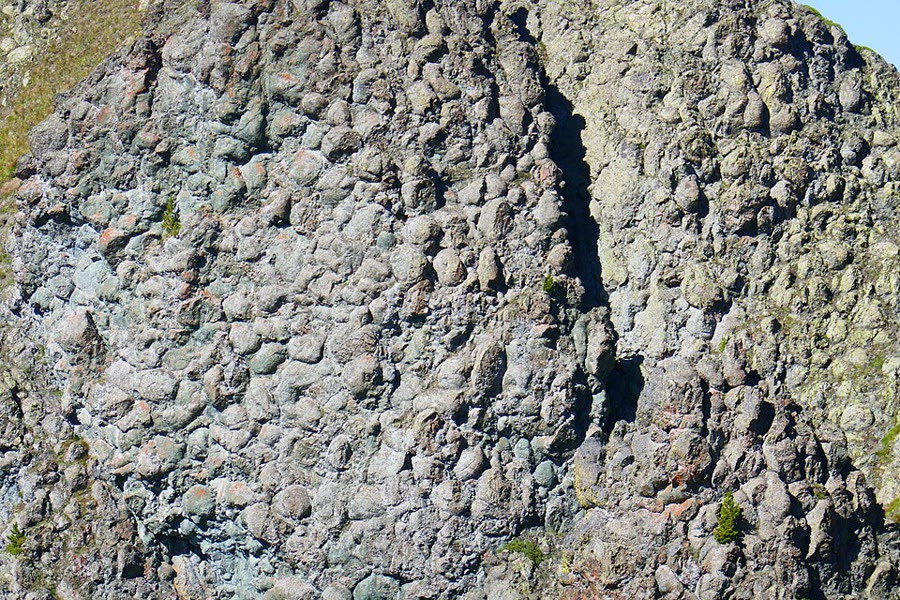
\includegraphics[width=0.66\linewidth]{images/book4/b2-13-pillow-lava.jpg}
\par\smallskip{\small Lava bantal \omterm{def:b2:alpine-orogen:ophiolite}{ofiolit} Chenaillet, Alpen Barat: setiap bantal yang membulat
adalah cuping basal yang meletus dan mendingin cepat di dasar samudra Piemont--Liguria.
Foto: Lionel Duchoiselle, CC BY-SA 3.0.}
\end{omfigure}

Dasar samudra dapat diberi umur di tempat gabronya mengkristal. Zirkon dari dua metagabro
\omterm{def:b2:alpine-orogen:ophiolite}{ofiolit} Zermatt--Saas, di bawah Matterhorn, memberikan $164.0 \pm \qty{2.7}{Ma}$ dan $163.5
\pm \qty{1.8}{Ma}$, dan sedimen kaya mangan yang diendapkan di atas basal berumur paling tua $161
\pm \qty{11}{Ma}$: dasar samudra Piemont--Liguria terbentuk pada Jura,
sekitar \qty{164}{Ma} yang lalu.
% ledger: rubatto98:zsf

\section{Menyubduksi samudra, lalu benua}\label{sec:b2:alpine-orogen:subduction}

Samudra menutup melalui subduksi. Akan tetapi, sebagian dasarnya berakhir di atas benua,
bukan di bawahnya, dan sebagian benua mengikuti samudra itu turun.

\begin{definition}[Obduksi; subduksi benua]\label{def:b2:alpine-orogen:obduction}
Yang disebut \emph{obduksi}\index{obduksi} adalah penempatan selembar litosfer samudra ke atas
tepi benua, dengan \omterm{def:b2:alpine-orogen:ophiolite}{ofiolit} menunggangi benua. Yang disebut \emph{subduksi
benua}\index{subduksi benua} adalah turunnya litosfer benua, yang ditarik
oleh slab samudra yang melekat padanya, ke dalam zona subduksi setelah samudra di depannya
habis.
\end{definition}

\omterm{def:b2:alpine-orogen:obduction}{Obduksi} terjadi di Dinarida, di tenggara Alpen: \omterm{def:b2:alpine-orogen:ophiolite}{ofiolit} samudra Vardar berumur Jura,
yang sendiri berumur Jura Tengah, tersesar-dorong pada Jura Akhir ke atas
baji akresi dan ke atas tepi Apulia. \omterm{def:b2:alpine-orogen:obduction}{Obduksi} lama dianggap juga telah menempatkan
\omterm{def:b2:alpine-orogen:ophiolite}{ofiolit} Chenaillet, karena batuannya hanya memperlihatkan \omterm{def:b2:metamorphic-facies:metamorphism}{metamorfisme} Alpen berderajat
sangat rendah. Sebuah studi baru-baru ini menemukan sisa lawsonit dan omfasit dalam gabro dan
albititnya, yang menempatkan puncak Alpennya pada 10 sampai \qty{11}{kbar} dan 340 sampai
\qty{360}{\celsius}: beban \omterm{def:b2:alpine-orogen:nappes}{tumpukan nappe} setebal sekitar 35 sampai \qty{40}{km}. Para penulisnya
menyimpulkan bahwa Chenaillet tersubduksi, bukan terobduksi, pengingat bahwa pembacaan
suatu \omterm{def:b2:alpine-orogen:ophiolite}{ofiolit} bertumpu pada sejarah \omterm{def:b2:metamorphic-facies:metamorphism}{metamorfismenya} sama besarnya dengan pada batuannya.
% ledger: schmid04:obduction, corno23:chenaillet

\subsection*{Samudra itu turun}

Pada Kapur, tepi selatan samudra Piemont--Liguria, yaitu tepi Apulia, menjadi
tepi aktif: paritnya terisi serpih dan batu pasir, yang kini menjadi sekis gampingan
yang disebut Bündnerschiefer atau schistes lustrés. Alpen timur juga merekam tumbukan
yang lebih awal, penutupan sebuah teluk samudra lain, Meliata, ke dalam Apulia, dengan
puncak tekanan tinggi sekitar \qty{100}{Ma}: Alpen adalah hasil dua orogenesis, yang satu
berumur Kapur dan yang lain berumur Tersier.
% ledger: schmid04:two-orogenies

\omterm{def:b2:alpine-orogen:ophiolite}{Ofiolit} Zermatt--Saas turun sampai fasies eklogit
\cref{ch:b2:metamorphic-facies}: eklogitnya mencapai 550 sampai \qty{600}{\celsius} dan 2.5 sampai
\qty{3.0}{GPa}, dan puncak tekanannya tercapai antara 48 dan \qty{44}{Ma}. Satu irisannya,
di Lago di Cignana, mengandung koesit dan intan mikroskopis dalam batuan yang semula berupa basal
dan sedimen dasar samudra; irisan itu mencapai sekitar \qty{615}{\celsius} dan \qty{2.8}{GPa}, dan
zirkonnya memberi umur titik terdalam itu $44.1 \pm \qty{0.7}{Ma}$. Dasar samudra yang lahir
\qty{164}{Ma} yang lalu tersubduksi, pada umur 120 juta tahun, sampai kedalaman
\qty{90}{km} atau lebih, lalu kembali.
% ledger: halama20:cignana, rubatto98:zsf

\subsection*{Benua menyusul}

Setelah samudra itu lenyap, tepi Eropa terseret mengikutinya. Kuarsit
yang mengandung koesit dari masif Dora Maira, yang dibahas dalam \cref{ch:b2:pt-paths}, adalah kerak benua
dari sisi Eropa samudra itu yang mencapai lebih dari \qty{90}{km}, sekitar
\qty{35}{Ma} yang lalu, dan kembali dengan kecepatan lempeng. Penentuan umur batuan tekanan tinggi
di sepanjang sabuk itu memberikan suatu urutan: tepi Apulia sendiri (zona Sesia) pada Kapur
Akhir, \omterm{def:b2:alpine-orogen:ophiolite}{ofiolit} samudra Piemont--Liguria pada sekitar \qty{44}{Ma}, dan
kerak benua Eropa pada Eosen akhir. Rubatto dan kawan-kawan membacanya sebagai tiga episode subduksi yang bergeser dalam waktu dari
tenggara ke barat laut, ke arah Eropa.
% ledger: chopin84:coesite, rh01:exhumation, rubatto98:zsf, ispra16:cervino

Tumbukan menyusul: samudra Valais, jalur samudra terakhir, menutup selama Eosen tengah sampai
akhir, dan sejak itu kerak benua ditumpuk di atas kerak benua.
Gambar di bawah merangkum urutan itu.
% ledger: schmid04:alpine-tethys

\begin{omfigure}
\centering
\begin{tikzpicture}[x=0.95cm, y=0.78cm, font=\scriptsize]
% (a) rifting and spreading
\begin{scope}[yshift=0cm]
\node[anchor=west, font=\scriptsize\bfseries] at (-0.2,0.75) {(a) Jura: samudra membuka};
\fill[gray!25] (0,0) -- (3.2,0) -- (3.8,-0.6) -- (0,-0.6) -- cycle;
\fill[gray!25] (6.2,0) -- (10,0) -- (10,-0.6) -- (5.6,-0.6) -- cycle;
\fill[omThm!35] (3.2,0) -- (6.2,0) -- (5.6,-0.6) -- (3.8,-0.6) -- cycle;
\fill[blue!8] (0,0) rectangle (10,0.4);
\draw[thick] (4.7,0) -- (4.7,-0.6);
\node at (1.6,-0.3) {Eropa};
\node at (8,-0.3) {Apulia};
\node[align=center] at (4.7,0.2) {punggungan};
\end{scope}
% (b) oceanic subduction
\begin{scope}[yshift=-1.7cm]
\node[anchor=west, font=\scriptsize\bfseries] at (-0.2,0.75) {(b) Kapur sampai Eosen: samudra tersubduksi};
\fill[blue!8] (0,0) rectangle (7,0.4);
\fill[gray!25] (0,0) -- (3.0,0) -- (3.6,-0.6) -- (0,-0.6) -- cycle;
\fill[omThm!35] (3.0,0) -- (6.3,0) -- (6.0,-0.5) -- (5.6,-0.95) -- (3.6,-0.6) -- cycle;
\fill[gray!25] (6.3,0) -- (6.6,0.3) -- (10,0.3) -- (10,-0.6) -- (6.4,-0.6) -- cycle;
\fill[omThm!35] (5.6,-0.95) -- (6.0,-0.5) -- (7.4,-1.3) -- (7.2,-1.55) -- cycle;
\fill[orange!40] (6.0,0) -- (6.3,0) -- (6.6,0.3) -- (6.35,0.3) -- cycle;
\draw[-{Latex[length=2mm]}] (7.0,-1.0) -- (7.6,-1.38);
\node at (1.6,-0.3) {Eropa};
\node at (8.4,-0.15) {Apulia};
\node[anchor=west] at (7.5,-1.1) {eklogit};
\end{scope}
% (c) continental subduction
\begin{scope}[yshift=-3.95cm]
\node[anchor=west, font=\scriptsize\bfseries] at (-0.2,0.75) {(c) Eosen: tepi Eropa menyusul};
\fill[gray!25] (0,0) -- (5.6,0) -- (6.2,-0.5) -- (7.4,-1.35) -- (7.1,-1.6) -- (5.6,-0.6) -- (0,-0.6) -- cycle;
\fill[omThm!35] (6.2,0.05) -- (6.6,0.3) -- (6.95,0.3) -- (6.4,-0.2) -- cycle;
\fill[gray!25] (6.6,0.3) -- (10,0.3) -- (10,-0.6) -- (6.9,-0.6) -- (6.4,-0.2) -- (6.95,0.3) -- cycle;
\draw[dashed] (6.6,-0.85) circle (0.22);
\draw (6.82,-0.9) -- (7.6,-1.2);
\node[anchor=west] at (7.6,-1.2) {kerak benua UHP};
\node at (2.4,-0.3) {Eropa};
\node at (8.4,-0.15) {Apulia};
\end{scope}
% (d) collision
\begin{scope}[yshift=-6.65cm]
\node[anchor=west, font=\scriptsize\bfseries] at (-0.2,1.4) {(d) Oligosen sampai kini: tumbukan, nappe, cekungan depan-pegunungan};
\fill[yellow!35] (0.6,0) -- (3.4,0) -- (3.4,-0.3) -- cycle;
\fill[gray!25] (0,-0.3) -- (3.4,-0.3) -- (4.2,0.5) -- (5.2,0.75) -- (6.2,0.55) -- (7.0,0.2) -- (10,0.2)
  -- (10,-0.7) -- (6.6,-0.7) -- (5.4,-1.5) -- (4.0,-1.5) -- (3.2,-0.9) -- (0,-0.9) -- cycle;
\draw (3.4,-0.3) -- (4.5,-1.0);
\draw (4.2,0.5) -- (5.6,-0.4);
\draw (5.2,0.75) -- (6.1,0.1);
\fill[omThm!35] (5.05,0.6) -- (5.55,0.68) -- (5.85,0.32) -- (5.4,0.25) -- cycle;
\fill[yellow!35] (7.0,0.2) -- (9.6,0.2) -- (7.0,-0.1) -- cycle;
\node at (1.4,-0.6) {Eropa};
\node at (8.6,-0.3) {Apulia};
\node[anchor=south] at (1.9,0.02) {molasse};
\node at (4.7,-1.25) {akar};
\node[anchor=south west] at (6.25,0.6) {tumpukan nappe};
\end{scope}
\end{tikzpicture}
\par\smallskip{\small Sejarah skematis Alpen, tidak berskala (litosfer samudra berwarna merah,
litosfer benua kelabu, baji akresi jingga, dan \omterm{def:b2:alpine-orogen:foreland}{cekungan depan-pegunungan} kuning).
(a)~Samudra Piemont--Liguria membuka di antara Eropa dan Apulia. (b)~Dasarnya tersubduksi
di bawah Apulia dan berubah menjadi eklogit. (c)~Tepi Eropa ikut tertarik turun dan
termetamorfosis pada tekanan ultratinggi. (d)~Kerak benua ditumpuk menjadi \omterm{def:b2:alpine-orogen:nappes}{nappe} di atas
akar yang menebal, dengan \omterm{def:b2:alpine-orogen:foreland}{cekungan depan-pegunungan} fleksural di kedua sisinya.}
\end{omfigure}
% ledger: schmid04:alpine-tethys, schmid04:two-orogenies, rubatto98:zsf, schmid04:foreland

\section{Nappe, klippe, dan jendela}\label{sec:b2:alpine-orogen:nappes}

Kepingan samudra dan benua tidak ditumpuk secara utuh. Kepingan itu dikerok sebagai irisan-irisan
tipis dan terbawa jauh.

\begin{definition}[Nappe; tumpukan nappe]\label{def:b2:alpine-orogen:nappes}
Yang disebut \emph{nappe}\index{nappe} adalah lembaran batuan yang besar, sering setebal beberapa kilometer dan sepanjang puluhan
kilometer, yang terbawa di sepanjang sesar dorong bersudut rendah atau di sayap terbalik lipatan
rebah yang besar jauh dari tempat asalnya; batuan suatu nappe bersifat
\emph{alokton}\index{alokton (satuan batuan)}, sedangkan batuan yang tetap di tempat bersifat
\emph{autokton}\index{autokton (satuan batuan)}. Yang disebut \emph{tumpukan
nappe}\index{tumpukan nappe} adalah tumpukan nappe yang nappe-nappenya yang secara struktur lebih tinggi
biasanya berasal dari bagian \omterm{def:b2:alpine-orogen:orogen}{orogen} yang lebih dalam.
\end{definition}

Di Alpen, urutan penumpukannya adalah geografi samudra yang lenyap itu dalam keadaan terbalik,
dan satuan-satuannya dinamai menurut asalnya (tabel di bawah).

\begin{omfigure}
\centering\small
\begin{tabular}{>{\raggedright\arraybackslash}p{0.24\linewidth}|>{\raggedright\arraybackslash}p{0.66\linewidth}}
satuan (atas ke bawah) & asal dan batuan \\ \hline
\omterm{def:b2:alpine-orogen:nappes}{Nappe} Austroalpin & tepi Apulia di utara Garis Periadriatik: irisan batuan dasar dan batuan
penutup yang terlepas dari kerak bawahnya \\
\omterm{def:b2:alpine-orogen:nappes}{Nappe} Margna--Sesia (zona Sesia, Dent Blanche) & kepingan yang terbelah lepas dari tepi
Apulia terluar ketika samudra membuka \\
\omterm{def:b2:alpine-orogen:nappes}{Nappe} Penninik Atas & samudra Piemont--Liguria: \omterm{def:b2:alpine-orogen:ophiolite}{ofiolit}, mantel tersingkap, sekis
gampingan \\
\omterm{def:b2:alpine-orogen:nappes}{Nappe} Penninik Tengah & benua pita Briançonnais \\
\omterm{def:b2:alpine-orogen:nappes}{Nappe} Penninik Bawah & samudra Valais: \omterm{def:b2:alpine-orogen:ophiolite}{ofiolit} dan sekis gampingan \\
\omterm{def:b2:alpine-orogen:nappes}{Nappe} Subpenninik & batuan dasar Eropa yang terlepas dari kerak bawahnya \\
\omterm{def:b2:alpine-orogen:nappes}{Nappe} Helvetik & penutup kaya batu gamping dari tepi Eropa dekat, yang terlepas dari
batuan dasarnya \\ \hline
Alpen Selatan & Apulia di selatan Garis Periadriatik: \omterm{def:b2:alpine-orogen:ftb}{sabuk lipatan--sesar dorong} bervergensi selatan,
sebagian besar berumur Miosen, setebal 10 sampai \qty{15}{km}
\end{tabular}
\par\smallskip{\small Satuan-satuan tektonik utama Alpen, dari puncak struktur
ke bawah, beserta domain asal masing-masing (menurut Schmid dan kawan-kawan).}
\end{omfigure}
% ledger: schmid04:units, schmid04:apulia

Lempeng atas, Apulia, terletak paling atas; di bawahnya menyusul, berurutan, samudra jauh,
Briançonnais, samudra dekat, dan tepi Eropa, dengan satuan terendah berupa satuan yang
dahulu paling dekat dengan Eropa. Lipatan-lipatan besar yang melipat ulang \omterm{def:b2:alpine-orogen:nappes}{nappe} setelah ditumpuk
kadang-kadang mengacaukan urutan itu, dan sebagian irisan, seperti Briançonnais, menghilang di sepanjang
sabuk.
% ledger: schmid04:units, schmid04:alpine-tethys

Erosi lalu memotong tumpukan itu, dan dua bentuk muncul pada peta.

\begin{definition}[Klippe; jendela tektonik]\label{def:b2:alpine-orogen:klippe}
Yang disebut \emph{klippe}\index{klippe} adalah sisa terpencil suatu \omterm{def:b2:alpine-orogen:nappes}{nappe}, yang
tertinggal berdiri di atas batuan di bawahnya ketika erosi telah menyingkirkan sisa lembarannya; klippe
dikelilingi oleh sesar dorong basalnya. Yang disebut \emph{jendela tektonik}\index{jendela tektonik} adalah lubang
yang tererosi menembus suatu \omterm{def:b2:alpine-orogen:nappes}{nappe}, tempat batuan di bawah sesar dorong basalnya tersingkap, dikelilingi oleh
\omterm{def:b2:alpine-orogen:nappes}{nappe} itu.
\end{definition}

\begin{omfigure}
\centering
\begin{tikzpicture}[x=0.68cm, y=0.68cm, font=\scriptsize]
\def\thrust{(0,0) -- (5,0) .. controls (6.5,0) and (7,1.1) .. (8,1.1)
  .. controls (9,1.1) and (9.5,0) .. (11,0) -- (16,0)}
\def\topo{(0,1.7) .. controls (3,1.9) and (5,1.8) .. (6,1.5) .. controls (7,1.0) .. (8,0.6)
  .. controls (9,1.0) .. (10.3,1.5) .. controls (11.3,1.3) .. (12.5,-0.4)
  .. controls (13.3,0.9) .. (14.5,0.95) .. controls (15.5,0.8) .. (16,-0.2)}
\begin{scope}
\clip \topo -- (16,-2.6) -- (0,-2.6) -- cycle;
\fill[gray!20] (0,-2.6) rectangle (16,2.2);
\fill[omThm!30] \thrust -- (16,2.2) -- (0,2.2) -- cycle;
\draw[gray!55, yshift=-0.9*0.68cm] \thrust;
\draw[gray!55, yshift=-1.8*0.68cm] \thrust;
\draw[line width=1.2pt] \thrust;
\end{scope}
\draw \topo;
\node at (2.5,1.0) {nappe};
\node[anchor=north west] at (0.2,-0.05) {sesar dorong basal};
\node at (3.6,-1.35) {autokton};
\draw[-{Latex[length=1.6mm]}] (8,2.0) node[anchor=south] {jendela tektonik} -- (8,0.75);
\draw[-{Latex[length=1.6mm]}] (14.5,2.0) node[anchor=south] {klippe} -- (14.5,1.05);
\end{tikzpicture}
\par\smallskip{\small Sebuah \omterm{def:b2:alpine-orogen:nappes}{nappe} (berwarna) di atas \omterm{def:b2:alpine-orogen:nappes}{autoktonnya} (kelabu) setelah erosi, dalam
penampang skematis: di tempat sesar dorong basalnya (garis tebal) melengkung ke atas, erosi telah memotong
\omterm{def:b2:alpine-orogen:nappes}{nappe} itu dan membuka \omterm{def:b2:alpine-orogen:klippe}{jendela tektonik} ke batuan di bawahnya; di depan, sisa
\omterm{def:b2:alpine-orogen:nappes}{nappe} berdiri terpencil di atas \omterm{def:b2:alpine-orogen:nappes}{autokton}, yaitu \omterm{def:b2:alpine-orogen:klippe}{klippe}.}
\end{omfigure}

Alpen penuh dengan keduanya. Matterhorn adalah sebuah \omterm{def:b2:alpine-orogen:klippe}{klippe}: puncaknya termasuk sistem sesar dorong Dent
Blanche, sebuah sisa batuan Apulia yang berdiri di atas seluruh baji, dengan
gneis dan gabro berumur Perm yang bertumpu di atas \omterm{def:b2:alpine-orogen:ophiolite}{ofiolit} \omterm{def:b2:alpine-orogen:nappes}{nappe} Zermatt--Saas
dan zona Combin, yang selanjutnya bertumpu di atas \omterm{def:b2:alpine-orogen:nappes}{nappe} Monte Rosa dan Grand St Bernard dari
sisi Eropa (foto di bawah). Di front utara
Alpen barat, \omterm{def:b2:alpine-orogen:nappes}{nappe} penutup dari bagian dalam sabuk membentuk Préalpes Romandes dan
\omterm{def:b2:alpine-orogen:klippe}{klippe} di Swiss tengah. Di Alpen timur, dua jendela terbuka menembus
tutup Austroalpin: jendela Engadine, tempat sekis samudra Valais dengan sekis biru tersingkap
di bawah sisa-sisa terakhir Briançonnais, dan jendela Tauern yang lebih besar, tempat
tepi Eropa dan irisan-irisan Tethys Alpen muncul dari bawah \omterm{def:b2:alpine-orogen:nappes}{nappe}
Austroalpin.
% ledger: ispra16:cervino, schmid04:windows

\begin{omfigure}
\centering
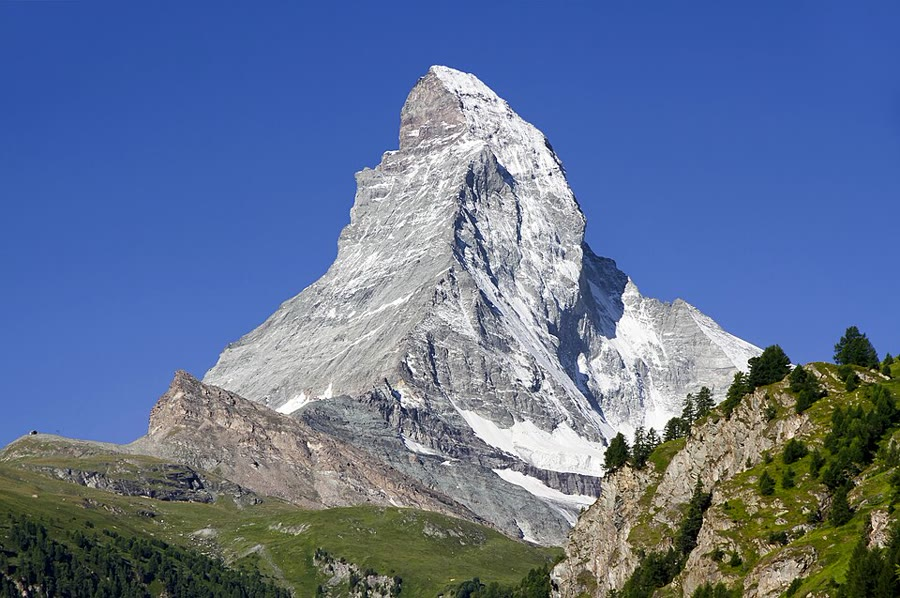
\includegraphics[width=0.7\linewidth]{images/book4/b2-13-matterhorn.jpg}
\par\smallskip{\small Sisi timur laut Matterhorn (\qty{4478}{m}), dilihat dari Zermatt:
piramida atasnya adalah gneis dan gabro Apulia dari sistem sesar dorong Dent Blanche, sebuah \omterm{def:b2:alpine-orogen:klippe}{klippe}
di atas \omterm{def:b2:alpine-orogen:ophiolite}{ofiolit} Tethys Alpen. Foto: Ximonic (Simo Räsänen), CC BY-SA
4.0.}
\end{omfigure}
% ledger: ispra16:cervino

\subsection*{Bidang lepasan dan dua kulit}

\omterm{def:b2:alpine-orogen:nappes}{Nappe} dan lembaran sesar dorong bergerak di atas bidang-bidang lemah.

\begin{definition}[Décollement]\label{def:b2:alpine-orogen:decollement}
Yang disebut \emph{décollement}\index{decollement@décollement} adalah bidang bersudut rendah tempat suatu
runtunan batuan terlepas dari batuan di bawahnya dan meluncur di atasnya, dengan kedua sisi terdeformasi
secara terpisah; bidang ini biasanya mengikuti lapisan lemah seperti evaporit atau serpih.
\end{definition}

\begin{definition}[Tektonik kulit tipis dan kulit tebal]\label{def:b2:alpine-orogen:skin}
Yang disebut \emph{tektonik kulit tipis}\index{tektonik kulit tipis} adalah deformasi penutup
sedimen yang terlepas dari batuan dasarnya di sepanjang \omterm{def:b2:alpine-orogen:decollement}{décollement} basal: penutup itu terlipat dan
tersesar-dorong sementara batuan dasar di bawahnya tetap tidak terdeformasi. Yang disebut \emph{tektonik kulit
tebal}\index{tektonik kulit tebal} adalah deformasi yang melibatkan batuan dasar,
dengan penutup dan batuan dasar memendek bersama pada sesar-sesar yang memotong ke dalam batuan dasar.
\end{definition}
% ledger: lanza22:jura

\begin{definition}[Sabuk lipatan--sesar dorong]\label{def:b2:alpine-orogen:ftb}
Yang disebut \emph{sabuk lipatan--sesar dorong}\index{sabuk lipatan--sesar dorong} adalah sabuk lipatan dan sesar dorong
yang memendekkan bagian luar suatu \omterm{def:b2:alpine-orogen:orogen}{orogen} dan merambat ke arah daratan depannya; sesar dorong
naik bertangga dari \omterm{def:b2:alpine-orogen:decollement}{décollement} menembus lapisan-lapisan, dan lipatan tumbuh di atasnya.
\end{definition}

Alpen memiliki kedua kulit. \omterm{def:b2:alpine-orogen:nappes}{Nappe} Helvetik adalah \omterm{def:b2:alpine-orogen:ftb}{sabuk lipatan--sesar dorong} kulit tipis,
batu gamping Mesozoikum tepi Eropa dekat yang terlepas dari batuan dasarnya. Dasarnya adalah
sesar dorong Glarus, tempat lapisan merah Perm terletak di atas \omterm{def:b2:alpine-orogen:foreland}{flysch} Kenozoikum. Sebaliknya, pada Miosen,
blok-blok batuan dasar masif eksternal, yaitu batuan dasar Eropa yang memendek dan menebal (masif
Aar, Mont Blanc, Belledonne, Pelvoux, dan Argentera), tersesar-dorong naik bersama
penutupnya: pensesaran dorong kulit tebal.
% ledger: schmid04:units, schmid04:skins, herwegh08:glarus, rosenberg21:massifs

Jura, busur punggungan di barat laut dataran Swiss, adalah contoh klasik kulit
tipis. Pada Miosen akhir dan Pliosen, penutup Mesozoikumnya terlipat dan tersesar-dorong di atas
\omterm{def:b2:alpine-orogen:decollement}{décollement} dalam evaporit Trias Tengah dan Atas yang lemah, sedangkan batuan dasar di bawahnya,
yang menerus dari masif eksternal di bawah Cekungan \omterm{def:b2:alpine-orogen:foreland}{Molasse}, tidak terlibat: menurut
pembacaan klasik, dorongannya berasal dari masif eksternal yang jauh. Seismologi sejak itu
menambahkan satu bab kulit tebal. Gempa bumi Saint-Ursanne pada 2000 bersumber
kurang dari satu kilometer di bawah permukaan dan bermekanisme sesar dorong, yaitu pensesaran dorong dangkal yang aktif di penutup,
sedangkan studi lain mendapati sesar batuan dasar yang teraktifkan kembali sejak Pliosen paling akhir. Apakah
Jura masih terlepas dari batuan dasarnya masih diperdebatkan.
% ledger: lanza22:jura, schmid04:skins

\begin{inthefield}[Membaca kontak sesar dorong]
Di antara Flims dan Walensee di Swiss timur membentang sesar dorong Glarus, salah satu
sesar dorong besar bersudut rendah yang paling menonjol di Alpen. Di sepanjangnya, lapisan merah Perm, yaitu
Verrucano, terletak di atas \omterm{def:b2:alpine-orogen:foreland}{flysch} Kenozoikum, batuan yang jauh lebih tua bertumpu di atas batuan yang lebih muda. Di antara keduanya, sebuah
pita batu gamping yang tipis dan tergerus kuat membentuk kontaknya: batu gamping Lochseiten, tempat pergeseran, sekurang-kurangnya 30 sampai
\qty{40}{km}, terpusat. Pada abad kesembilan belas, Heim membaca struktur itu sebagai dua lipatan
rebah raksasa yang saling berhadapan; Escher von der Linth telah membacanya sebagai satu sesar sungkup, dan pembacaan sesar dorong itulah yang menang. Ahli geologi yang menjumpai kontak semacam itu memeriksa
tiga hal: apakah batuan yang lebih tua terletak di atas batuan yang lebih muda, yang tidak mungkin terjadi pada perlapisan biasa;
apakah lapisan di kedua sisi terpancung pada kontak itu; dan apakah kontak itu
sendiri berupa pita batuan yang tergerus dan terekristalisasi, bukan bidang perlapisan.
\end{inthefield}
% ledger: herwegh08:glarus

\section{Cekungan depan-pegunungan: flysch dan molasse}\label{sec:b2:alpine-orogen:foreland}

Sabuk pegunungan membebani lempeng yang ditungganginya, dan lempeng itu melengkung turun di depannya.

\begin{definition}[Cekungan depan-pegunungan; flysch; molasse]\label{def:b2:alpine-orogen:foreland}
Yang disebut \emph{cekungan depan-pegunungan}\index{cekungan depan-pegunungan} adalah cekungan sedimen memanjang yang terbentuk
di antara suatu \omterm{def:b2:alpine-orogen:orogen}{orogen} dan benua stabil di depannya, tempat lempeng dilengkungkan turun oleh
beban baji sesar dorong; cekungan ini paling dalam di dekat front sesar dorong dan lambat laun ikut
tertindih sesar dorong. Yang disebut \emph{flysch}\index{flysch} adalah isian air dalam cekungan
semacam itu, terutama turbidit batu pasir dan serpih yang diendapkan selagi cekungan kurang terisi.
Yang disebut \emph{molasse}\index{molasse} adalah isian laut dangkal dan isian kontinental yang menyusul kemudian, terutama
konglomerat dan batu pasir dari sabuk yang tererosi, yang diendapkan setelah pasokan mengisi
cekungan.
\end{definition}
% ledger: sinclair97:trinity, schmid04:foreland, krenmayr99:molasse

Pelengkungan itu adalah fleksur elastis litosfer, yang dibahas dalam salah satu bab volume Tahun 3;
di sini hanya pengaruhnya pada cekungan yang penting. Sinclair menggambarkan \omterm{def:b2:alpine-orogen:foreland}{cekungan depan-pegunungan} Alpen awal, yang berumur Paleosen sampai Oligosen,
sebagai ``trinitas kurang terisi'': batu gamping di sisi benua, lumpur hemipelagis di
tengah, turbidit air dalam di depan front sesar dorong. Ketika sesar dorong maju, cekungan itu
ikut berpindah: di Swiss, garis pantai kontinentalnya bergeser perlahan ke barat laut dengan laju 8.5
sampai \qty{12.9}{mm} per tahun, dan cekungan itu bermigrasi dengan bentuk yang hampir tetap sejauh sekurang-kurangnya
\qty{210}{km} di atas lempeng Eropa.
% ledger: sinclair97:trinity

Cekungan \omterm{def:b2:alpine-orogen:foreland}{Molasse} Alpen utara, yang membentang dari Alpen Maritim sampai Wina, mulai
turun pada Eosen akhir. \omterm{def:b2:alpine-orogen:foreland}{Flysch} Oligosen Bawah, yang kini dijumpai di atas \omterm{def:b2:alpine-orogen:nappes}{nappe}
Helvetik, merekam tahap air dalam terakhir; dari Oligosen akhir sampai Miosen akhir, sungai-sungai
menyebarkan kerikil dan pasir kontinental dari pegunungan muda itu. Namanya sudah tua: H.-B. de Saussure
memperkenalkan \emph{\omterm{def:b2:alpine-orogen:foreland}{molasse}} pada 1779. Isiannya menebal ke arah sabuk: di
sektor Austria, sampai lebih dari \qty{4000}{m} di front sesar dorong, dan di tempat lain dalam cekungan itu
satu rangkaian konglomerat sungai berumur Oligosen akhir saja setebal sekitar \qty{4}{km}. Bagian selatan
cekungan itu telah tertindih: sabuk singkapan Austria, selebar sekitar \qty{60}{km}, kurang
dari seperempat lebar cekungan semula. \omterm{def:b2:alpine-orogen:foreland}{Molasse} yang tertindih itu sendiri terperangkap dalam
sesar dorong sebagai \omterm{def:b2:alpine-orogen:foreland}{Molasse} Subalpin, irisan-irisan konglomerat yang miring ke selatan di sepanjang
tepi utara sabuk.
% ledger: schmid04:foreland, krenmayr99:molasse, gs18:conglomerates

Di selatan Alpen, Dataran Po terletak di atas daratan depan Adriatik Alpen Selatan yang hanya sedikit
terdeformasi. Sedimennya yang termuda, berumur Pliosen dan Pleistosen, sebagian menutupi struktur
Alpen secara tidak selaras dan sebagian terdeformasi oleh sesar dorong terakhir Alpen Selatan
dan Apennina.
% ledger: schmid04:foreland

\begin{omfigure}
\centering
\begin{tikzpicture}[x=0.5cm, y=0.6cm, font=\scriptsize]
\begin{scope}
\node[anchor=west, font=\scriptsize\bfseries] at (0,2.4) {(a) kurang terisi: flysch};
\fill[blue!8] (0,0) -- (12,0) -- (12,1.4) -- (9.0,1.4) -- (4,0.05) -- (0,0.05) -- cycle;
\fill[gray!25] (0,0) -- (12,-1.1) -- (12,-1.9) -- (0,-0.8) -- cycle;
\fill[omThm!30] (9.0,1.4) -- (12,2.2) -- (12,-1.1) -- (9.5,-0.87) -- cycle;
\fill[green!25!gray!40] (5.5,-0.5) -- (9.5,-0.87) -- (9.3,-0.35) -- (7.0,-0.2) -- cycle;
\node at (10.9,0.6) {baji};
\node at (2,-0.45) {kraton};
\node[anchor=north] at (7.3,-0.9) {turbidit};
\draw[->] (7.3,-0.95) -- (7.6,-0.55);
\end{scope}
\begin{scope}[xshift=6.4cm]
\node[anchor=west, font=\scriptsize\bfseries] at (0,2.4) {(b) terisi berlebih: molasse};
\fill[gray!25] (0,0) -- (12,-1.1) -- (12,-1.9) -- (0,-0.8) -- cycle;
\fill[omThm!30] (8.5,1.6) -- (12,2.4) -- (12,-1.1) -- (9.0,-0.82) -- cycle;
\fill[yellow!40] (1.5,-0.13) -- (9.0,-0.82) -- (8.5,1.0) -- (5,0.35) -- cycle;
\fill[blue!8] (0,0) -- (1.5,-0.13) -- (5,0.35) -- (4,0.4) -- (0,0.4) -- cycle;
\node at (10.6,0.6) {baji};
\node at (2,-0.45) {kraton};
\node at (6.2,-0.05) {kerikil, pasir};
\end{scope}
\end{tikzpicture}
\par\smallskip{\small \omterm{def:b2:alpine-orogen:foreland}{Cekungan depan-pegunungan} dalam dua tahap (skematis). (a)~Pada awalnya, lempeng yang melengkung
turun lebih cepat daripada datangnya sedimen: air dalam di depan baji sesar dorong, tempat
turbidit (\omterm{def:b2:alpine-orogen:foreland}{flysch}) berakumulasi. (b)~Kemudian sabuk yang tererosi memasok lebih banyak daripada yang dapat
ditampung cekungan: sungai-sungai mengisinya dengan kerikil dan pasir (\omterm{def:b2:alpine-orogen:foreland}{molasse}), dan baji itu tersesar-dorong di atas
rombakannya sendiri.}
\end{omfigure}
% ledger: sinclair97:trinity, schmid04:foreland

\section{Membaca sejarahnya: penampang dan geofisika}\label{sec:b2:alpine-orogen:sections}

Peta menunjukkan letak satuan-satuan; penampang menunjukkan bagaimana satuan-satuan itu terletak di bawah permukaan, dan penampang dapat
diuji.

\begin{definition}[Penampang seimbang]\label{def:b2:alpine-orogen:balanced}
Yang disebut \emph{penampang seimbang}\index{penampang seimbang} adalah penampang batuan
terdeformasi, yang digambar sejajar arah transpor, yang dapat dipulihkan ke keadaan tak terdeformasi
yang masuk akal secara geologis tanpa menambah atau kehilangan batuan: panjang lapisan penanda dan
luas satuan batuan dalam penampang itu kekal antara keadaan terdeformasi dan keadaan
yang dipulihkan.
\end{definition}

Pemulihannya dijangkarkan oleh \emph{garis pin}, garis-garis yang melintang lapisan di kedua ujung
penampang, yang dipilih di tempat batuan tidak saling tergelincir.

\begin{proposition}[Neraca panjang garis dan neraca luas]\label{prop:b2:alpine-orogen:balance}
Di antara dua garis pin yang berjarak $l$ dalam keadaan terdeformasi, misalkan suatu lapisan penanda memiliki
panjang $l_0$ yang diukur di sepanjang lapisan itu, dan misalkan suatu lapisan dengan tebal semula $t$ memiliki
luas penampang $A$. Jika panjang dan luas kekal pada bidang penampang,
\begin{enumerate}
\item lapisan itu sepanjang $l_0$ sebelum deformasi, pemendekannya
$e = 1 - l/l_0$ dan jarak pemendekannya $S = l_0 - l$;
\item panjang pulihan lapisan itu $l_0 = A/t$;
\item jika suatu horizon penanda terletak pada kedalaman $d$ di atas \omterm{def:b2:alpine-orogen:decollement}{décollement} yang datar, luas batuan
yang terangkat di atas aras semula penanda itu, yaitu \emph{luas lebih}-nya $A_e$, sama dengan $S\,d$;
karena itu $d = A_e/S$.
\end{enumerate}
\end{proposition}

\begin{omfigure}
\centering
% book's own geometry (figdata/bachelor-2/alps.py)
\begin{tikzpicture}
\begin{axis}[width=0.86\linewidth, height=4.0cm, axis equal image, xmin=-1.5, xmax=31.5,
  ymin=-7.5, ymax=4.8, axis lines=none, clip=false]
\addplot[omThm, line width=1.2pt] table[x=x_km, y=y_km] {figdata/out/bachelor-2-alps-chevron.dat};
\addplot[gray, line width=1.2pt] table[x=x_km, y=y_km] {figdata/out/bachelor-2-alps-chevron0.dat};
\draw[dashed] (axis cs:0,-7) -- (axis cs:0,4.3);
\draw[dashed] (axis cs:22.98,-1.2) -- (axis cs:22.98,4.3);
\draw[dashed] (axis cs:30,-7) -- (axis cs:30,-4.8);
\draw[<->] (axis cs:0,-1.4) -- node[below, font=\scriptsize] {$l = \qty{23.0}{km}$} (axis cs:22.98,-1.4);
\node[font=\scriptsize, anchor=south] at (axis cs:15,-5.9) {dipulihkan: $l_0 = \qty{30.0}{km}$};
\node[font=\scriptsize, anchor=west] at (axis cs:23.3,2.2) {kemiringan sayap \qty{40}{\degree}};
\node[font=\scriptsize, anchor=south] at (axis cs:0,4.3) {pin};
\node[font=\scriptsize, anchor=south] at (axis cs:22.98,4.3) {pin};
\end{axis}
\end{tikzpicture}
\par\smallskip{\small Neraca panjang garis sebuah lapisan penanda yang terlipat menjadi lipatan chevron dengan sayap
miring \qty{40}{\degree} (atas), dan lapisan yang sama yang dipulihkan di antara garis-garis pinnya
(bawah), pada skala sebenarnya. Setiap sayap mempertahankan panjangnya; lapisan yang terlipat membentang
$l = 30.0\cos\qty{40}{\degree} = \qty{23.0}{km}$, pemendekan sebesar $1 - \cos\qty{40}{\degree} =
\qty{23.4}{\percent}$.}
\end{omfigure}

\begin{proof}
(1) Lapisan yang tidak meregang maupun memendek di sepanjang panjangnya mempertahankan panjang itu; pemendekan adalah
fraksi panjang yang hilang, seperti di sekolah. (2) Sebelum deformasi, lapisan itu berupa jalur sepanjang
$l_0$ dan setebal $t$, dengan luas $l_0 t$, dan luas itu kekal. (3) Sebelum
deformasi, batuan di antara aras penanda dan \omterm{def:b2:alpine-orogen:decollement}{décollement} mengisi jalur sepanjang $l_0$
dan setebal $d$. Sesudahnya, di antara garis-garis pin, batuan yang sama mengisi jalur sepanjang $l$
dari \omterm{def:b2:alpine-orogen:decollement}{décollement} sampai aras semula penanda, dengan luas $l\,d$, ditambah luas lebih
yang terdorong di atas aras itu. Kekekalan memberikan $l_0 d = l\,d + A_e$, sehingga $A_e = (l_0 -
l)\,d = S\,d$. Relasi itu memberikan kedalaman \omterm{def:b2:alpine-orogen:decollement}{décollement} yang tersembunyi dari luas lebih
dan pemendekan yang terukur.
\end{proof}


\begin{method}[Memulihkan penampang]\label{met:b2:alpine-orogen:restore}
\begin{enumerate}
\item Pilihlah penampang yang sejajar arah transpor dan dua garis pin di tempat yang tidak mengalami
gelinciran antarlapisan.
\item Ukurlah setiap lapisan penanda di sepanjang panjangnya di antara kedua pin, dengan menghitung setiap bagian
yang terulang oleh sesar dorong.
\item Bentangkan lapisan-lapisan itu secara datar dengan panjang terukurnya, dengan mempertahankan urutan lapisan,
lalu gambarkan ulang sesar-sesar pada penampang pulihan: potongan-potongannya harus segaris, tanpa celah
atau tumpang-tindih.
\item Bandingkan: lapisan-lapisan dari lembaran sesar dorong yang sama harus pulih ke panjang yang sama; luas
lapisan-lapisan, dibagi tebalnya, juga harus memberikan panjang yang sama. Penampang yang
gagal tidak dapat diterima sebagaimana digambar.
\end{enumerate}
\end{method}

Penyeimbangan adalah uji atas suatu penampang, bukan buktinya, dan asumsi-asumsinya penting. Di Jura
dekat Chasseral, penyeimbangan panjang garis puncak Jura memberikan pergeseran \qty{5.1}{km},
tetapi penyeimbangan luas dan pemodelan maju memberikan \qty{11.3}{km}: tambahan
\qty{6.2}{km} itu terbawa di sepanjang bidang lepasan kedua yang lebih atas dalam serpih Jura dan diteruskan
ke lipatan-lipatan lebih jauh ke utara. Satu lapisan penanda telah melewatkan separuh gerakannya. Studi yang sama
menimbang, dan tidak memerlukan, dua pembacaan lain yang lazim di Jura: tinggian batuan dasar yang mendorong
lipatan ke atas, dan inti antiklin yang menebal oleh evaporit Trias yang mengalir ke dalamnya, suatu
proses yang menggagalkan neraca luas, karena lapisan evaporit tidak lagi mempertahankan
tebalnya.
% ledger: schori15:chasseral, schori15:evaporite-flow

\subsection*{Berapa besar pemendekannya?}

Bila diterapkan pada seluruh lintasan, penyeimbangan memberikan pemendekan total sabuk itu, dan jawabannya
berbeda menurut asumsinya. Di Alpen Tengah, di sepanjang lintasan NFP-20, taksiran
pemendekan tumbukan adalah sekitar \qty{125}{km} dalam karya-karya awal, \qty{160}{km} dalam
kompilasi 2015, dan \qty{144}{km} dalam tinjauan 2021; penambahan gelinciran dekstral pada Garis Periadriatik, yang
menggeser Apulia ke samping di sepanjang sabuk, menaikkan konvergensi total menjadi antara 206 dan
\qty{250}{km}, bergantung pada besarnya gelinciran yang diandaikan. Di Alpen Barat, taksirannya
berkisar dari 124 sampai \qty{243}{km}. Setiap taksiran itu adalah jumlah kepingan-kepingan yang dipulihkan, masing-masing dengan
garis pin sendiri dan dugaan sendiri tentang apa yang telah disingkirkan erosi dan subduksi.
% ledger: rosenberg21:shortening

\subsection*{Apa yang dilihat geofisika}

Penampang di kedalaman bertumpu pada geofisika. Profil refleksi seismik dalam telah ditembakkan
melintasi sabuk itu (ECORS--CROP di Alpen Barat, NFP-20 Barat dan Timur di
Swiss, TRANSALP di timur), dan jaringan seismometer yang rapat kini memetakan Moho
dari fungsi penerima, yaitu konversi gelombang P teleseismik menjadi gelombang S di dasar
kerak. Peta AlpArray, yang dibangun dari lebih dari seratus ribu fungsi penerima,
mendapati Moho pada sekitar \qty{30}{km}, khas benua, di sekeliling sabuk, dan pada 55 sampai
\qty{60}{km} di bawah Alpen; Moho Eropa miring landai dari sekitar \qty{30}{km} di
barat laut sampai sekitar \qty{55}{km} di bawah jajaran pegunungan itu.
Penampang skematis di bawah merangkum cara membaca profil-profil NFP-20 yang melintasi Alpen Tengah.
% ledger: schmid04:transects, michailos23:moho

\begin{omfigure}
\centering
\begin{tikzpicture}[x=0.6cm, y=0.5cm, font=\scriptsize]
% surface and cover
\fill[yellow!30] (0,0) -- (3.0,0) -- (6.5,-0.3) -- (8.0,0.4) -- (8.0,-0.9) -- (0,-0.6) -- cycle;
\fill[gray!12] (0,-0.6) -- (8.0,-0.9) -- (12.5,-4.5) -- (15,-3.5) -- (16.5,-6.6) -- (16,-8.3)
  -- (0,-5.0) -- cycle;
\fill[gray!35] (0,-5.0) -- (16,-8.3) -- (17.5,-10.0) -- (0,-6.0) -- cycle;
% Helvetic and Aar
\fill[cyan!25] (8.0,0.4) -- (10.0,1.6) -- (11.0,1.2) -- (9.5,-0.4) -- (8.0,-0.9) -- cycle;
\fill[gray!12] (8.0,-0.9) -- (9.5,-0.4) -- (11.0,1.2) -- (12.0,2.0) -- (12.8,0.2) -- (11.5,-1.8)
  -- (12.5,-4.5) -- cycle;
% Penninic stack
\fill[omThm!35] (12.0,2.0) -- (14.5,2.6) -- (17.0,2.2) -- (17.3,-1.0) -- (15.0,-3.5) -- (12.5,-4.5)
  -- (11.5,-1.8) -- (12.8,0.2) -- cycle;
% Austroalpine/Apulia and Southern Alps
\fill[orange!30] (17.0,2.2) -- (19.0,1.6) -- (24,0.2) -- (26,0) -- (26,-3.5) -- (20.5,-4.0)
  -- (17.3,-1.0) -- cycle;
\fill[brown!35] (17.3,-1.0) -- (20.5,-4.0) -- (19.0,-7.0) -- (16.5,-6.6) -- (15,-3.5) -- cycle;
\fill[gray!35] (20.5,-4.0) -- (26,-3.5) -- (26,-6.0) -- (19.0,-7.0) -- cycle;
\fill[yellow!30] (23.5,0.3) -- (26,0) -- (26,-0.5) -- (24.5,-0.3) -- cycle;
\draw[thick] (17.3,-1.0) -- (17.0,2.2);
\draw[thick] (8.0,-0.9) -- (12.5,-4.5);
\draw[dashed] (0,-6.0) -- (17.5,-10.0);
\draw[dashed] (19.0,-7.0) -- (26,-6.0);
\node at (2.2,-0.25) {Jura};
\node at (5.2,-0.35) {molasse};
\node at (9.0,0.15) {Helvetik};
\node at (10.6,-0.6) {Aar};
\node at (14.6,0.4) {nappe Penninik};
\node at (21.2,-0.9) {Alpen Selatan};
\node at (24.9,-0.3) {Po};
\node at (18.0,-4.8) {Ivrea};
\node[align=center] at (5,-3.0) {kerak Eropa};
\node[anchor=north] at (3.2,-7.4) {Moho Eropa};
\node at (10,-9.3) {mantel};
\node at (23,-7.7) {mantel};
\node[anchor=north] at (23,-6.55) {Moho Adriatik};
\node[anchor=south, align=center] at (17.2,2.25) {Garis\\Periadriatik};
\draw[-{Latex[length=2mm]}] (1.0,0.5) -- (0.0,0.5);
\node[anchor=south] at (0.5,0.5) {BL};
\draw[-{Latex[length=2mm]}] (25.0,1.2) -- (26.0,1.2);
\node[anchor=south] at (25.5,1.2) {TG};
\end{tikzpicture}
\par\smallskip{\small Penampang kerak skematis yang melintasi Alpen Tengah, dari Jura sampai
Dataran Po (tidak berskala; menurut tafsiran lintasan-lintasan NFP-20 yang dikompilasi oleh
Schmid dan kawan-kawan). Kerak Eropa, dengan Jura yang terlipat lepas dari bagian atasnya, menunjam di bawah
\omterm{def:b2:alpine-orogen:nappes}{nappe} Helvetik, masif Aar, dan \omterm{def:b2:alpine-orogen:nappes}{tumpukan nappe} Penninik; di selatan Garis
Periadriatik, kerak Apulia dengan baji tubuh Ivrea terletak di atas Moho Eropa, dan
Alpen Selatan tersesar-dorong ke selatan di atas Dataran Po.}
\end{omfigure}
% ledger: schmid04:transects, schmid04:units, schmid04:apulia, schmid04:skins


\begin{omfigure}
\centering
% ledger: data:b4-etopo-alps, data:b4-alps-moho, michailos23:moho
\begin{tikzpicture}
\begin{groupplot}[group style={group size=1 by 2, vertical sep=0.25cm, x descriptions at=edge bottom},
  width=0.92\linewidth, xmin=0, xmax=300, tick label style={font=\scriptsize},
  label style={font=\small}]
\nextgroupplot[height=3.6cm, ymin=0, ymax=4000, ylabel={elevasi (\unit{m})},
  ytick={0,1000,2000,3000,4000}, y tick label style={/pgf/number format/1000 sep={}},
  legend style={font=\scriptsize, at={(0.99,0.97)}, anchor=north east, draw=none, fill=none}]
\addplot[gray, line width=0.4pt] table[x=km, y=max_m] {figdata/out/bachelor-2-alps-swath.dat};
\addplot[omThm, line width=1pt] table[x=km, y=mean_m] {figdata/out/bachelor-2-alps-swath.dat};
\legend{maksimum jalur, rata-rata jalur}
\node[font=\scriptsize, anchor=south west] at (axis cs:2,2650) {A (Dataran Po)};
\node[font=\scriptsize, anchor=south east] at (axis cs:298,1500) {B};
\nextgroupplot[height=4.6cm, ymin=0, ymax=70, y dir=reverse, xlabel={jarak ke utara dari
  \qty{45.3}{\degree} LU di sepanjang \qty{8}{\degree} BT (\unit{km})}, ylabel={kedalaman (\unit{km})},
  legend style={font=\scriptsize, at={(0.99,0.03)}, anchor=south east, draw=none, fill=none}]
\addplot[only marks, mark=*, mark size=1.6pt, black] table[x=km, y=moho_km] {figdata/out/bachelor-2-alps-moho.dat};
\addplot[omThm, dashed, line width=0.8pt] table[x=km, y=airy_km] {figdata/out/bachelor-2-alps-airy.dat};
\addplot[gray, densely dotted] coordinates {(0,30) (300,30)};
\legend{Moho terbaca, prediksi Airy, \qty{30}{km}}
\end{groupplot}
\end{tikzpicture}
\par\smallskip{\small Profil A--B di sepanjang \qty{8}{\degree} BT. Atas: elevasi rata-rata dan maksimum
simpul ETOPO1 dalam jalur selebar \qty{0.25}{\degree} di kedua sisi meridian itu.
Bawah: kedalaman Moho yang dibaca pada meridian ini dalam peta fungsi penerima AlpArray
(Michailos dan kawan-kawan, CC BY 4.0), dan Moho yang akan ditempatkan isostasi Airy lokal di bawah
relief rata-rata jalur, untuk kerak \qty{30}{km} dan massa jenis 2700 dan
\qty{3300}{kg.m^{-3}}.}
\end{omfigure}

Profil di atas mengonfrontasikan akar itu dengan model Airy dari volume
Tahun 1. Di bawah bagian tertinggi profil, tempat relief rata-rata jalur mencapai
\qty{2.74}{km} pada \qty{46.5}{\degree} LU, akar Airy lokal akan menempatkan Moho pada
$30 + 4.5 \times 2.74 = \qty{42.3}{km}$; Moho teramati pada \qty{36.3}{km}. Sekitar seratus
kilometer lebih ke selatan, di tepi Dataran Po, tempat relief rata-ratanya hanya
\qty{0.65}{km}, Moho yang teramati adalah yang terdalam pada profil itu, \qty{61.2}{km}. Akar itu tidak berada di bawah puncak-puncak: akar itu
bergeser ke arah Apulia. Pada bentangan yang memiliki titik bacaan, luas penampangnya, yang diukur
di bawah \qty{30}{km}, sekitar \qty{2300}{km^2}, dibandingkan dengan sekitar \qty{1500}{km^2} untuk akar
Airy relief di atasnya. Kompensasi lokal topografi masa kini tidak
menjelaskan akar itu. Pfiffner dan kawan-kawan menunjuk beban tambahan: tubuh Ivrea, baji
mantel dan kerak bawah Adriatik di dalam sabuk itu, yang ikut melengkungkan lempeng Eropa
ke bawah.
% ledger: data:b4-etopo-alps, data:b4-alps-moho, michailos23:moho, pfiffner02:ivrea

Gravitasi menceritakan kisah yang sama dengan cara lain. Peta anomali Bouguer seluruh Alpen memperlihatkan
rendahan gravitasi Alpen sebesar $-100$ sampai \qty{-170}{mGal} di sepanjang jajaran pegunungan, paling dalam di Alpen
Tengah, dari kerak ringan akar yang menebal; rendahan cekungan Po sekitar $-80$ sampai
\qty{-140}{mGal}; dan, di antara Alpen Barat dan Dataran Po, tinggian gravitasi Ivrea
yang sempit, sampai \qty{+40}{mGal}, tempat kerak bawah dan mantel yang rapat itu mendekati
permukaan.
% ledger: zahorec21:gravity

\section{Garis waktu Alpen}\label{sec:b2:alpine-orogen:timeline}

Dengan mengumpulkan tanggal-tanggal bab ini, diperoleh sejarah sabuk itu dalam satu tabel
(tabel di bawah).

\begin{omfigure}
\centering\small
\begin{tabular}{p{0.28\linewidth}|p{0.62\linewidth}}
waktu & peristiwa \\ \hline
Jura Tengah & samudra Piemont--Liguria membuka; gabronya mengkristal pada
\qty{164}{Ma} \\
Kapur paling awal & samudra Valais membuka di utara Briançonnais \\
sekitar \qty{100}{Ma} & puncak tekanan tinggi orogenesis Kapur di Alpen timur \\
Kapur Akhir & tepi Apulia (zona Sesia) tersubduksi; tepi Apulia
samudra itu aktif \\
48 sampai \qty{44}{Ma} & dasar samudra Zermatt--Saas mencapai titik terdalamnya, koesit dan
intan di Lago di Cignana \\
Eosen tengah sampai akhir & samudra Valais menutup; Cekungan \omterm{def:b2:alpine-orogen:foreland}{Molasse} mulai turun \\
\qty{35}{Ma} & kerak benua Dora Maira pada tekanan ultratinggi \\
Oligosen dan Miosen & sesar dorong Glarus; kerikil \omterm{def:b2:alpine-orogen:foreland}{molasse} mengisi daratan depan utara (Oligosen
akhir sampai Miosen akhir) \\
Miosen & pengangkatan kulit tebal masif eksternal; Alpen Selatan tersesar-dorong
ke selatan \\
Miosen akhir sampai Pliosen & pelipatan kulit tipis Jura \\
kini & pengukuran sipat datar menunjukkan pengangkatan batuan relatif sampai \qty{1.3}{mm} per tahun di inti
Alpen Tengah
\end{tabular}
\par\smallskip{\small Alpen dalam sebelas langkah; sumber-sumbernya dikutip dalam subbab-subbab
di atas.}
\end{omfigure}
% ledger: schmid04:alpine-tethys, rubatto98:zsf, schmid04:two-orogenies, halama20:cignana, schmid04:foreland, rh01:exhumation, herwegh08:glarus, schmid04:skins, schmid04:apulia, champagnac09:uplift

Baris terakhir itu bukan akhir konvergensi. Pengukuran sipat datar berulang di Alpen Tengah
memberikan pengangkatan batuan relatif dari sekitar \qty{-0.4}{mm} per tahun di utara Jura sampai
\qty{1.3}{mm} per tahun di inti jajaran pegunungan, sedangkan pengukuran GPS menunjukkan bahwa
Alpen Tengah tidak sedang berkonvergensi saat ini. Champagnac dan kawan-kawan membaca pengangkatan itu sebagai pantulan isostatik
kerak yang bebannya berkurang oleh erosi: pegunungan naik karena pegunungan itu terkikis.
% ledger: champagnac09:uplift

\section*{Latihan}\label{sec:b2:alpine-orogen:exercises}

Data untuk latihan: $g = \qty{9.8}{m.s^{-2}}$,
$G = \qty{6.674e-11}{m^3.kg^{-1}.s^{-2}}$.

\begin{exercise}[$\star$]\label{exo:b2:alpine-orogen:1}
Dalam sebuah penampang, suatu lapisan batu gamping yang diukur di sepanjang lipatannya di antara dua garis pin
panjangnya \qty{36.0}{km}; kedua garis pin itu berjarak \qty{27.0}{km}. (a) Dengan
\cref{prop:b2:alpine-orogen:balance}, hitunglah pemendekan $e$ dan jarak pemendekan
$S$. (b) Apa yang harus berlaku pada lapisan itu agar jawabannya sahih?
\end{exercise}

\begin{exercise}[$\star$]\label{exo:b2:alpine-orogen:2}
Pada sebuah peta geologi, (a) sebidang gneis berbentuk lonjong sepanjang \qty{4}{km} terletak di atas batu gamping
Jura, dengan batas berupa sesar dorong yang miring ke dalam, ke bawah gneis, di sekelilingnya; (b) suatu
daerah memanjang serpih Kapur dikelilingi gneis, di sepanjang sesar dorong yang miring
ke luar, ke bawah gneis, di sekelilingnya. Namailah setiap struktur dan jelaskan apa yang telah dilakukan erosi
dalam setiap kasus.
\end{exercise}

\begin{exercise}[$\star$]\label{exo:b2:alpine-orogen:3}
(a) Sebutkan keempat satuan \omterm{def:b2:alpine-orogen:ophiolite}{sekuen ofiolit Penrose} dari bawah ke atas, dan pasangkan masing-masing
dengan satu lapisan kerak samudra atau mantel. (b) \omterm{def:b2:alpine-orogen:ophiolite}{Ofiolit} Chenaillet memperlihatkan mantel
tersingkap, gabro, dan basal bantal, tanpa penutup sedimen. Satuan Penrose mana yang tidak ada dalam
daftar ini? (c) Mengapa \omterm{def:b2:alpine-orogen:ophiolite}{ofiolit} tidak memberikan sampel yang mewakili dasar samudra-samudra
luas?
\end{exercise}
% ledger: coleman84:penrose, coleman84:settings, corno23:chenaillet

\begin{exercise}[$\star$]\label{exo:b2:alpine-orogen:4}
Dalam pendakian Matterhorn dari selatan, seorang pendaki berturut-turut melintasi \omterm{def:b2:alpine-orogen:nappes}{nappe} Monte Rosa dan
Grand St Bernard, \omterm{def:b2:alpine-orogen:ophiolite}{ofiolit} Zermatt--Saas, zona Combin, dan gneis
sistem sesar dorong Dent Blanche. (a) Sebutkan domain asal masing-masing. (b) Lempeng mana yang menjadi
lempeng atas selama subduksi? (c) Mengapa urutan ini menjadi aturan umum dalam \omterm{def:b2:alpine-orogen:nappes}{tumpukan nappe},
dan apa yang dapat merusaknya?
\end{exercise}
% ledger: ispra16:cervino, schmid04:units

\begin{exercise}[$\star\star$]\label{exo:b2:alpine-orogen:5}
Alpen Tengah memiliki anomali Bouguer sekitar \qty{-170}{mGal}. (a) Dengan lempeng
Bouguer dari volume Tahun 1, $\Delta g = 2\pi G\,\Delta\rho\,h$, tentukan tebal $h$ lempeng
tak hingga dengan defisit massa jenis $\Delta\rho = \qty{500}{kg.m^{-3}}$ (kerak menggantikan mantel)
yang memberikan anomali ini. (b) Fungsi penerima menunjukkan akar sekitar \qty{25}{km} di bawah kerak
\qty{30}{km}. Anomali berapa yang akan diberikan lempeng tak hingga setebal itu? (c) Mengapa
anomali teramati lebih kecil?
\end{exercise}
% ledger: zahorec21:gravity, michailos23:moho

\begin{exercise}[$\star\star$]\label{exo:b2:alpine-orogen:6}
Gabro \omterm{def:b2:alpine-orogen:ophiolite}{ofiolit} Zermatt--Saas mengkristal pada \qty{164}{Ma}; \omterm{def:b2:alpine-orogen:ophiolite}{ofiolit} itu mencapai
titik terdalamnya pada \qty{44}{Ma}, pada \qty{2.8}{GPa}. (a) Berapa umur litosfer samudra
itu ketika tersubduksi? (b) Ubahlah tekanan itu menjadi kedalaman dengan massa jenis rata-rata batuan di atasnya
\qty{3000}{kg.m^{-3}}, lalu \qty{3300}{kg.m^{-3}}. (c) Bandingkan dengan
``lebih dari \qty{90}{km}'' yang dikutip untuk batuan ini.
\end{exercise}
% ledger: rubatto98:zsf, halama20:cignana

\begin{exercise}[$\star\star$]\label{exo:b2:alpine-orogen:7}
Suatu lapisan terlipat menjadi lipatan chevron yang sayap-sayap lurusnya semuanya miring dengan sudut $\theta$.
(a) Tunjukkan bahwa pemendekannya $e = 1 - \cos\theta$. (b) Kemiringan sayap berapa yang memberikan
pemendekan \qty{30}{\percent}? (c) Pemendekan berapa yang diberikan sayap yang miring \qty{40}{\degree} dan
\qty{60}{\degree}? Periksalah hasil pertama dengan gambar lipatan chevron pada subbab tentang penyeimbangan.
\end{exercise}

\begin{exercise}[$\star\star$]\label{exo:b2:alpine-orogen:8}
Penutup setebal \qty{2.0}{km} terlipat dan tersesar-dorong di atas \omterm{def:b2:alpine-orogen:decollement}{décollement} yang datar. Di antara garis-garis pin
yang kini berjarak \qty{42}{km}, luas penampangnya \qty{118}{km^2}. (a) Tentukan panjang
pulihannya, $S$, dan $e$. (b) Hitunglah luas lebih dan kedalaman \omterm{def:b2:alpine-orogen:decollement}{décollement} di bawah
puncak semula penutup itu. (c) Apakah hasilnya konsisten?
\end{exercise}

\begin{exercise}[$\star\star$]\label{exo:b2:alpine-orogen:9}
Di sepanjang profil \qty{8}{\degree} BT bab ini, elevasi rata-rata jalur adalah
\qty{2.74}{km} pada \qty{46.5}{\degree} LU, tempat Moho terbaca pada \qty{36.3}{km}, dan
\qty{0.65}{km} pada \qty{45.55}{\degree} LU, tempat Moho terbaca pada \qty{61.2}{km}. (a) Dengan
kerak acuan \qty{30}{km}, $\rho_c = \qty{2700}{kg.m^{-3}}$, dan $\rho_m =
\qty{3300}{kg.m^{-3}}$, hitunglah kedalaman Moho Airy di kedua tempat. (b) Bandingkan dengan
nilai terbaca. (c) Apa yang dikatakan perbandingan itu tentang cara akar Alpen ditopang?
\end{exercise}
% ledger: data:b4-etopo-alps, data:b4-alps-moho, pfiffner02:ivrea

\begin{exercise}[$\star\star\star$]\label{exo:b2:alpine-orogen:10}
Pada penampang Chasseral di Jura, penyeimbangan panjang garis puncak Jura
memberikan pergeseran \qty{5.1}{km}; penyeimbangan luas dan pemodelan memberikan \qty{11.3}{km}, dan
\qty{6.2}{km} di antaranya terbawa di sepanjang bidang lepasan atas dalam serpih Jura Tengah.
(a) Berapa fraksi pergeseran yang direkam lapisan puncak Jura? (b) Tunjukkan bahwa
angka-angka itu cocok jumlahnya, dan jelaskan mengapa lapisan atas melewatkan sebagian gerakan. (c) Pelajaran
umum apa yang diberikannya untuk penyeimbangan dengan satu lapisan penanda?
\end{exercise}
% ledger: schori15:chasseral

\begin{exercise}[$\star\star\star$]\label{exo:b2:alpine-orogen:11}
Di Alpen Tengah, pemendekan berarah utara sekitar \qty{200}{km} telah
ditaksir, dan Garis Periadriatik memiliki pergeseran dekstral barat--timur sekitar
\qty{100}{km}, mungkin 50, mungkin 150. (a) Jumlahkan keduanya sebagai vektor yang saling tegak lurus dan berikan
konvergensi total untuk setiap pergeseran. (b) Berapa sudut yang dibentuk konvergensi itu dengan
arah utara--selatan untuk pergeseran \qty{100}{km}? (c) Mengapa pilihan pergeseran
lebih penting daripada angka penting ketiga pemendekan?
\end{exercise}
% ledger: rosenberg21:shortening

\begin{exercise}[$\star\star\star$]\label{exo:b2:alpine-orogen:12}
Bagian Swiss \omterm{def:b2:alpine-orogen:foreland}{cekungan depan-pegunungan} Alpen bermigrasi sekurang-kurangnya \qty{210}{km} ke barat laut
di atas Eropa, dengan garis pantainya maju 8.5 sampai \qty{12.9}{mm} per tahun. (a) Dalam rentang
durasi berapa migrasi itu berlangsung? (b) Di sektor Austria, sabuk singkapan masa kini,
selebar sekitar \qty{60}{km}, kurang dari seperempat lebar cekungan semula. Berapa
lebar semula terkecilnya, dan berapa bagian cekungan yang tersembunyi di bawah sesar dorong? (c) Mengapa
\omterm{def:b2:alpine-orogen:foreland}{cekungan depan-pegunungan} tidak pernah dapat terawetkan sepenuhnya?
\end{exercise}
% ledger: sinclair97:trinity, krenmayr99:molasse

\begin{problem}[{Soal akhir pekan --- memulihkan penampang}]\label{pb:b2:alpine-orogen:1}
Sebuah \omterm{def:b2:alpine-orogen:orogen}{orogen} bertipe Alpen dilintasi oleh penampang model (geometri rekaan, buatan buku ini sendiri,
yang ditandai sebagai model) yang terdiri atas lima domain, dari daratan depan ke sisi jauh:
\omterm{def:b2:alpine-orogen:ftb}{sabuk lipatan--sesar dorong} daratan depan, kini selebar \qty{48}{km}; \omterm{def:b2:alpine-orogen:nappes}{tumpukan nappe} eksternal, \qty{15}{km};
masif batuan dasar, \qty{22}{km}; zona internal berupa \omterm{def:b2:alpine-orogen:nappes}{nappe} benua dan \omterm{def:b2:alpine-orogen:ophiolite}{ofiolit},
\qty{20}{km}; dan baji belakang bervergensi selatan, \qty{48}{km}
(gambar di bawah). Semua panjang dinyatakan dalam kilometer.

\begin{omfigure}
\centering
\begin{tikzpicture}[x=0.075cm, y=0.5cm, font=\scriptsize]
\fill[yellow!30] (0,0) rectangle (48,1);
\fill[cyan!25] (48,0) rectangle (63,1);
\fill[gray!25] (63,0) rectangle (85,1);
\fill[omThm!35] (85,0) rectangle (105,1);
\fill[orange!30] (105,0) rectangle (153,1);
\draw (0,0) rectangle (153,1);
\foreach \x in {48,63,85,105} \draw (\x,0) -- (\x,1);
\node at (24,0.5) {sabuk daratan depan};
\node[align=center] at (55.5,1.6) {nappe};
\node at (74,0.5) {masif};
\node[align=center] at (95,1.6) {internal};
\node at (129,0.5) {baji belakang};
\node[anchor=north] at (24,0) {48}; \node[anchor=north] at (55.5,0) {15};
\node[anchor=north] at (74,0) {22}; \node[anchor=north] at (95,0) {20};
\node[anchor=north] at (129,0) {48};
\end{tikzpicture}
\par\smallskip{\small Penampang model soal akhir pekan: lebar masa kini kelima
domainnya, dalam kilometer (seluruhnya 153; geometri rekaan).}
\end{omfigure}

\noindent\textbf{Bagian I --- Neraca panjang garis sabuk daratan depan.} Di antara kedua garis
pinnya, yang berjarak \qty{48.0}{km}, puncak batu gamping utama terdiri atas sepuluh ruas lurus
(bentang horizontal $\Delta x$, kemiringan), yang didaftar dari daratan depan; selain itu, selembar sesar dorong
menutupi bentangan datar lapisan yang sama, sepanjang \qty{6.0}{km}, yang terulang di bawahnya.

\smallskip
\begin{center}\small
\begin{tabular}{l|cccccccccc}
ruas & 1 & 2 & 3 & 4 & 5 & 6 & 7 & 8 & 9 & 10\\ \hline
$\Delta x$ (\unit{km}) & 8.0 & 3.0 & 3.0 & 5.0 & 2.5 & 2.5 & 6.0 & 4.0 & 4.0 & 10.0\\
kemiringan (\unit{\degree}) & 0 & 35 & 35 & 0 & 50 & 50 & 10 & 40 & 40 & 5
\end{tabular}
\end{center}
\smallskip

\begin{enumerate}
\item Hitunglah panjang di sepanjang lapisan untuk ruas 2, 5, dan 8.
\item Hitunglah panjang total lapisan di antara garis-garis pin, termasuk bentangan yang
terulang.
\item Mengapa bentangan yang tersembunyi di bawah lembaran sesar dorong harus dihitung?
\item Hitunglah pemendekan $e$ dan jarak pemendekan $S$ sabuk daratan depan.
\item Dasar batu gamping, yang diukur dengan cara yang sama, panjangnya \qty{60.2}{km}. Berapa besar,
dan berapa persen, selisih kedua lapisan itu? Apakah penampang itu dapat diterima?
\item Apa artinya jika panjang dasar itu \qty{54.0}{km}?
\end{enumerate}

\noindent\textbf{Bagian II --- Neraca luas dan décollement.} Penutup di antara
\omterm{def:b2:alpine-orogen:decollement}{décollement} dan puncak batu gamping setebal \qty{2.4}{km} sebelum deformasi; luasnya
di antara garis-garis pin terukur \qty{146}{km^2}.
\begin{enumerate}[resume]
\item Hitunglah panjang pulihan penutup itu dari luasnya.
\item Bandingkan dengan hasil panjang garis pertanyaan~2.
\item Hitunglah luas lebih, yang terangkat di atas puncak semula penutup.
\item Turunkan kedalaman \omterm{def:b2:alpine-orogen:decollement}{décollement} di bawah aras itu, dan bandingkan dengan tebal
penutup.
\item Seandainya luasnya \qty{160}{km^2}, panjang pulihan berapa yang akan diberikannya? Proses mana,
yang disebut dalam pembahasan Jura, yang dapat membuat luas dan panjang garis berselisih seperti itu?
\item Mengapa sabuk ini berkulit tipis, dan seperti apa seharusnya puncak batuan dasar
di bawahnya?
\end{enumerate}

\noindent\textbf{Bagian III --- Nappe eksternal dan lajunya.} Lapisan penanda
ketiga \omterm{def:b2:alpine-orogen:nappes}{nappe} eksternal pulih menjadi 22, 18, dan \qty{25}{km}; tumpukan itu kini membentang
\qty{15}{km}. Di masif batuan dasar, puncak batuan dasar pulih menjadi \qty{30}{km}
dibandingkan dengan \qty{22}{km} kini. Sabuk daratan depan terdeformasi antara 11 dan \qty{4}{Ma}, sedangkan
\omterm{def:b2:alpine-orogen:nappes}{nappe} antara 30 dan \qty{20}{Ma}.
\begin{enumerate}[resume]
\item Hitunglah panjang pulihan \omterm{def:b2:alpine-orogen:nappes}{tumpukan nappe} dan jarak pemendekannya.
\item Hitunglah pemendekannya $e$ dan bandingkan dengan pemendekan sabuk daratan depan.
\item Hitunglah pemendekan masif batuan dasar. Tektonik jenis apakah ini?
\item Hitunglah laju pemendekan rata-rata sabuk daratan depan dan \omterm{def:b2:alpine-orogen:nappes}{nappe}, dalam
milimeter per tahun.
\item Ke arah mana deformasi bermigrasi di sepanjang penampang? Apakah ini urutan
di Alpen?
\item Jumlahkan pemendekan ketiga domain eksternal.
\end{enumerate}

\noindent\textbf{Bagian IV --- Zona internal, samudra, dan seluruh penampang.}
Irisan-irisan \omterm{def:b2:alpine-orogen:ophiolite}{ofiolit} di zona internal pulih menjadi \qty{18}{km}. Andaikan samudra itu
tersubduksi dari 85 sampai \qty{45}{Ma} dengan laju rata-rata \qty{0.5}{cm} per tahun. \omterm{def:b2:alpine-orogen:nappes}{Nappe}
benua zona internal pulih menjadi \qty{60}{km} dibandingkan dengan \qty{20}{km} kini, dan
lapisan penanda baji belakang menjadi \qty{70}{km} dibandingkan dengan \qty{48}{km}.
\begin{enumerate}[resume]
\item Berapa panjang litosfer samudra yang tersubduksi?
\item Berikan lebar minimum samudra itu.
\item Mengapa nilai itu hanya minimum?
\item Hitunglah pemendekan zona internal dan baji belakang.
\item Jumlahkan pemendekan tumbukan kelima domain, dan bandingkan dengan
taksiran untuk Alpen Tengah dalam bab ini.
\item Pemeriksaan kerak: pulihkan penampang itu ke lebar penuhnya dengan kerak \qty{30}{km}, lalu
bandingkan luas keraknya dengan luas masa kini, yaitu rata-rata \qty{45}{km} sepanjang
\qty{153}{km} sekarang. Berapa fraksi kerak yang hilang dari penampang masa kini, dan ke mana
kerak itu pergi? Berikan pemendekan tumbukan total di sepanjang penampang, dibulatkan sampai
kilometer.
\end{enumerate}
\end{problem}
